\section{Parallelization}
\label{sec:md_parallelization}
Da parallelization technique is straight-up similar ta what tha fuck our phat asses did up in DSMC up in section \ref{sec:dmsc_parallelization}. Da spatial domain is divided tha fuck into $P_x\times P_y\times P_z$ smalla domains ($P_i$ bein tha number of processors up in tha $i$th dimension). Each such domain is then of size $l_x\times l_y \times l_z$ where $l_i = L_i/P_i$. Da processor arrangement n' labelin is done as shown up in figure \ref{fig:md_parallelization_2}, where a processor wit coordinates $(p_x, p_y, p_z)$ controls atoms wit coordinates up in tha range
\begin{align}
	\nonumber
	x&\in[p_xl_x, (p_x+1)l_x\rangle\\
	\nonumber
	y&\in[p_yl_y, (p_y+1)l_y\rangle\\
	z&\in[p_zl_z, (p_z+1)l_z\rangle.
\end{align}
\begin{figure}[h!]
\begin{center}
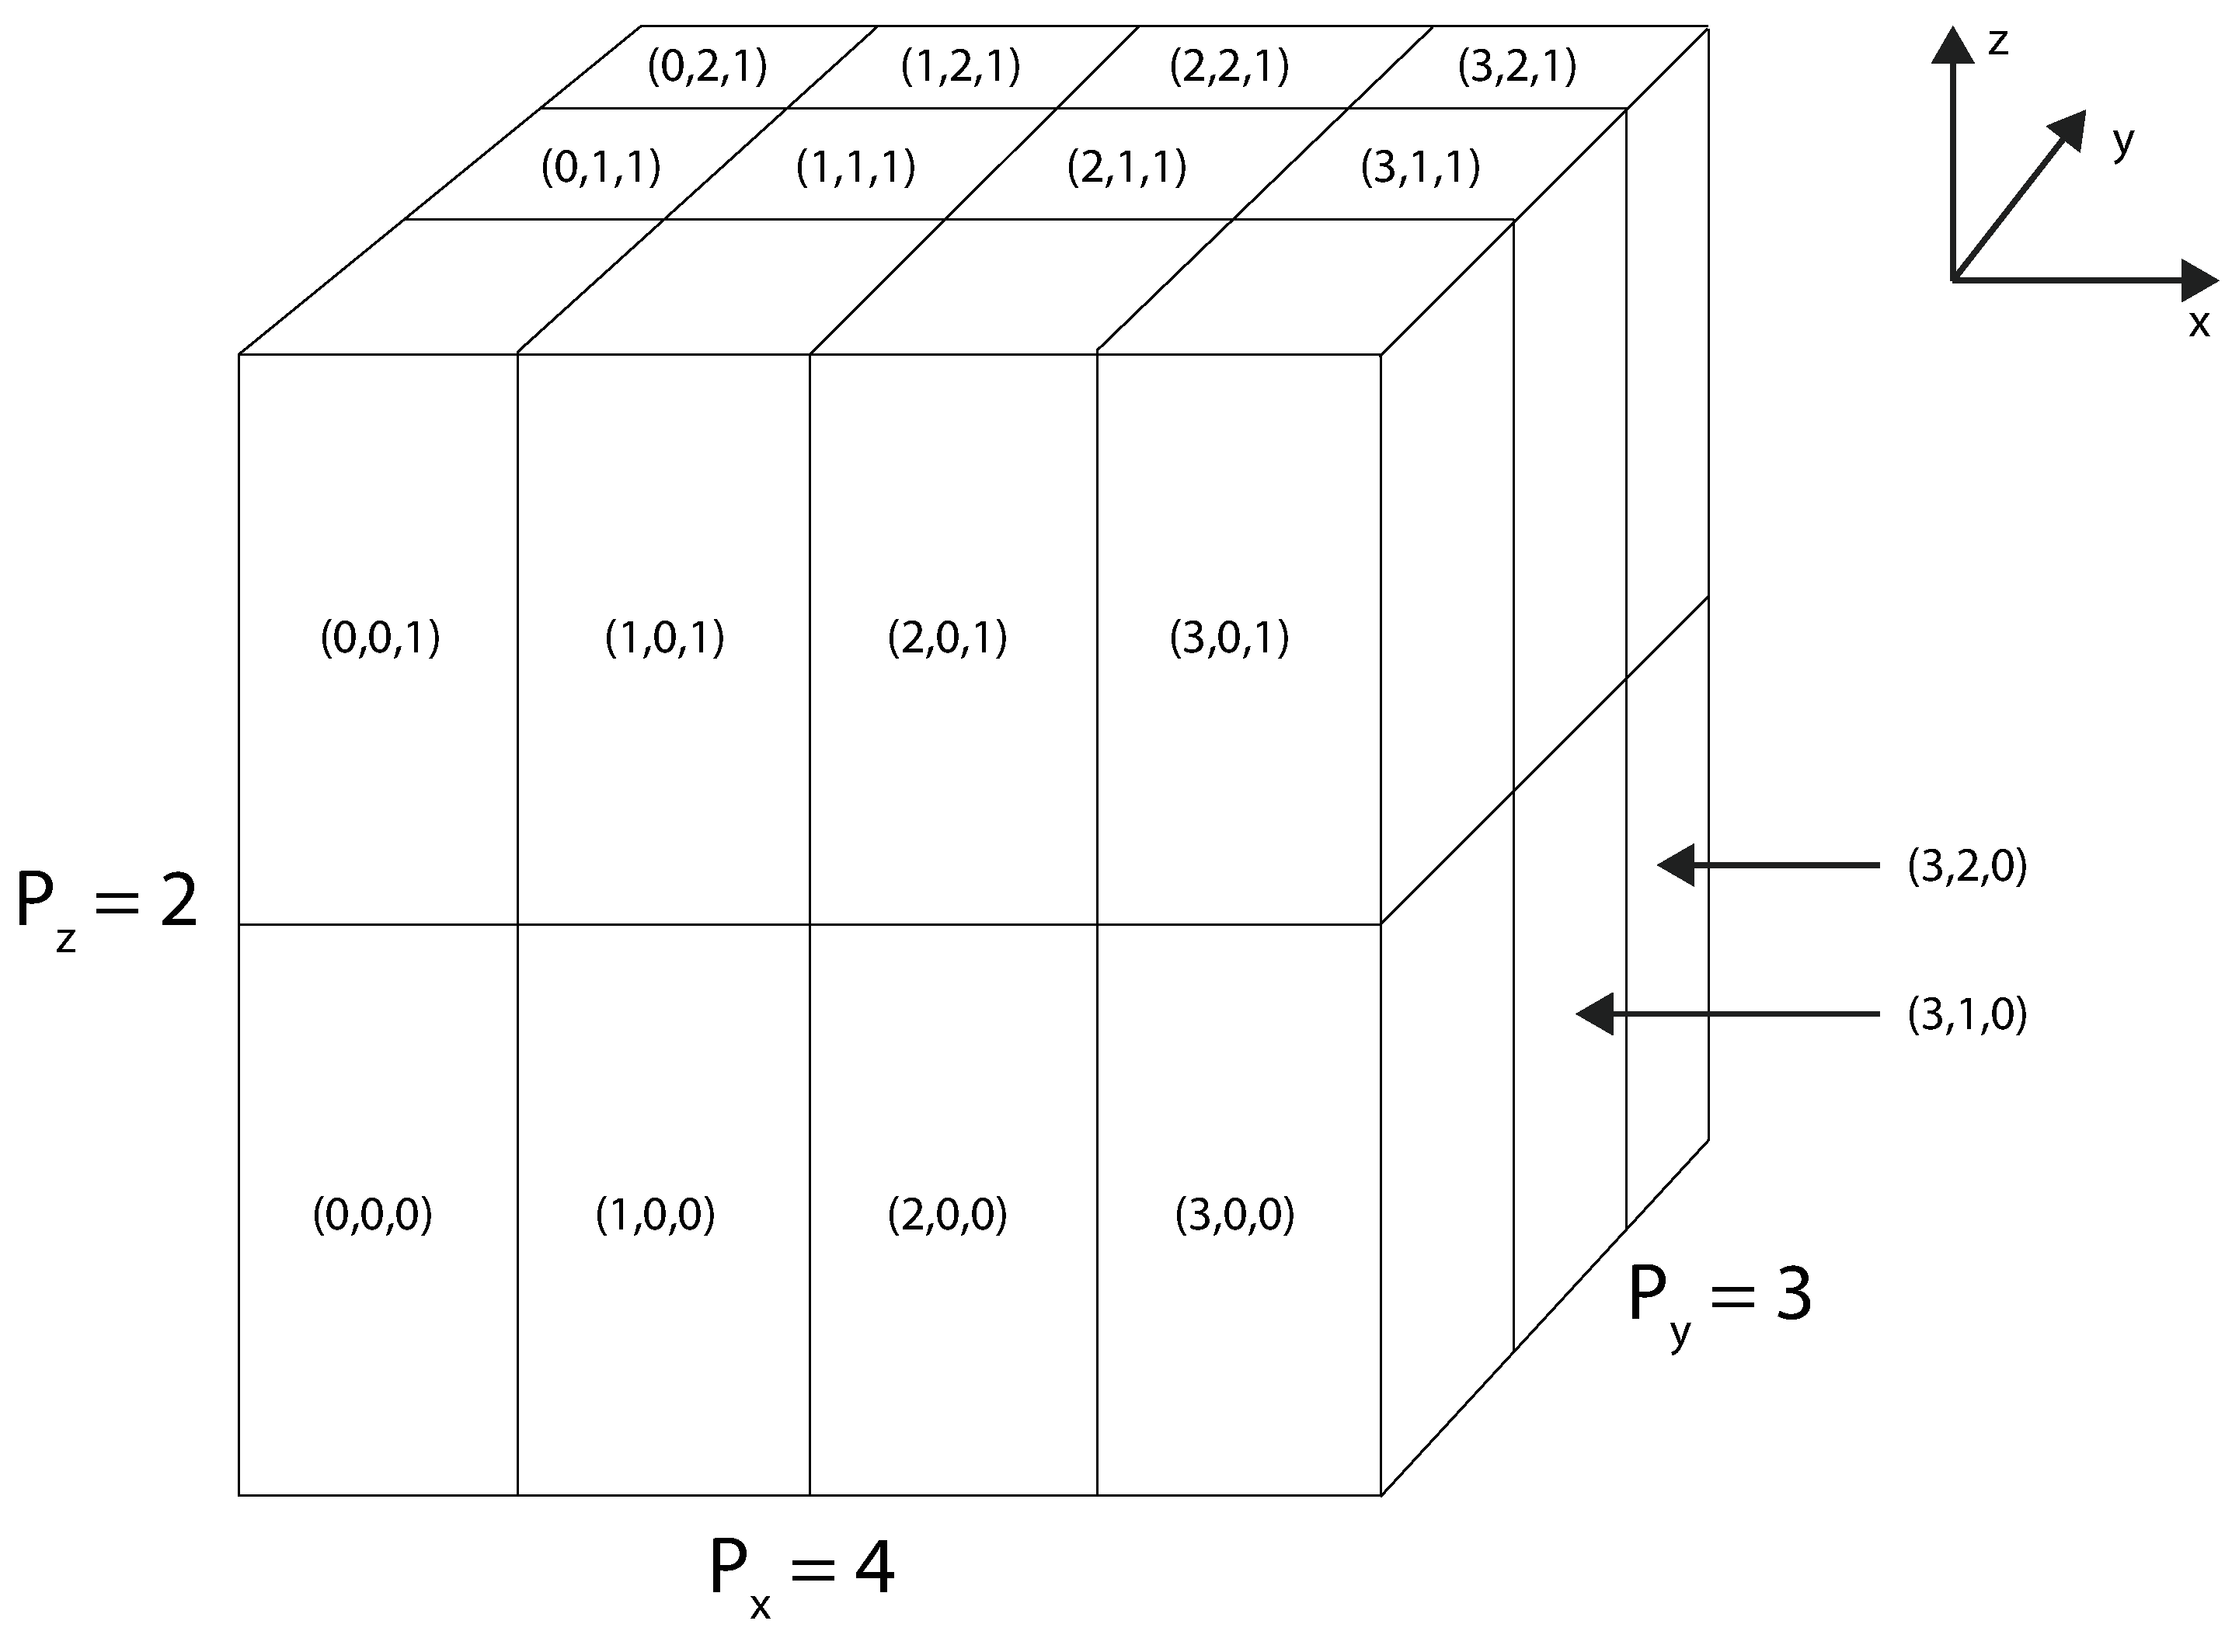
\includegraphics[width=0.7\textwidth, trim=0cm 0cm 0cm 0cm, clip]{DSMC/figures/parallelization_node_configuration.eps}
\end{center}
\caption{Processor labelin up in a 3-dimensionizzle grid. Y'all KNOW dat shit, muthafucka! Each processor is uniquely identified all up in its coordinizzle $(p_x, p_y, p_z)$.}
\label{fig:md_parallelization_2}
\end{figure}
We represent tha coordinatez of a atom on processor $(p_x, p_y, p_z)$ up in tha local coordinizzle system where tha CPUz origin $\vec p_\text{origin}$ defines tha coordinizzle system fo' realz. An atom wit global coordinates $\vec r$ will then have local coordinates $\vec r'$
\begin{align}
	\vec r' = \vec r - \vec p_\text{origin}.
\end{align}
We can then easily detect if a atom has moved outside its processorz domain by checkin if any of tha local coordinizzle components is outside tha range $[0, l_i)$ fo' dimension $i$. If a atom has moved ta another processor, it has moved ta one of tha 26 neighborin processors. Us thugs will use tha same 3-step process as busted lyrics bout up in subsection \ref{sec:dsmc_parallelization_exchange_particles} which is dopest illustrated wit tha 2-dimensionizzle example up in figure \ref{fig:md_parallelization_facet_technique}.
\begin{figure}[h!]
\begin{center}
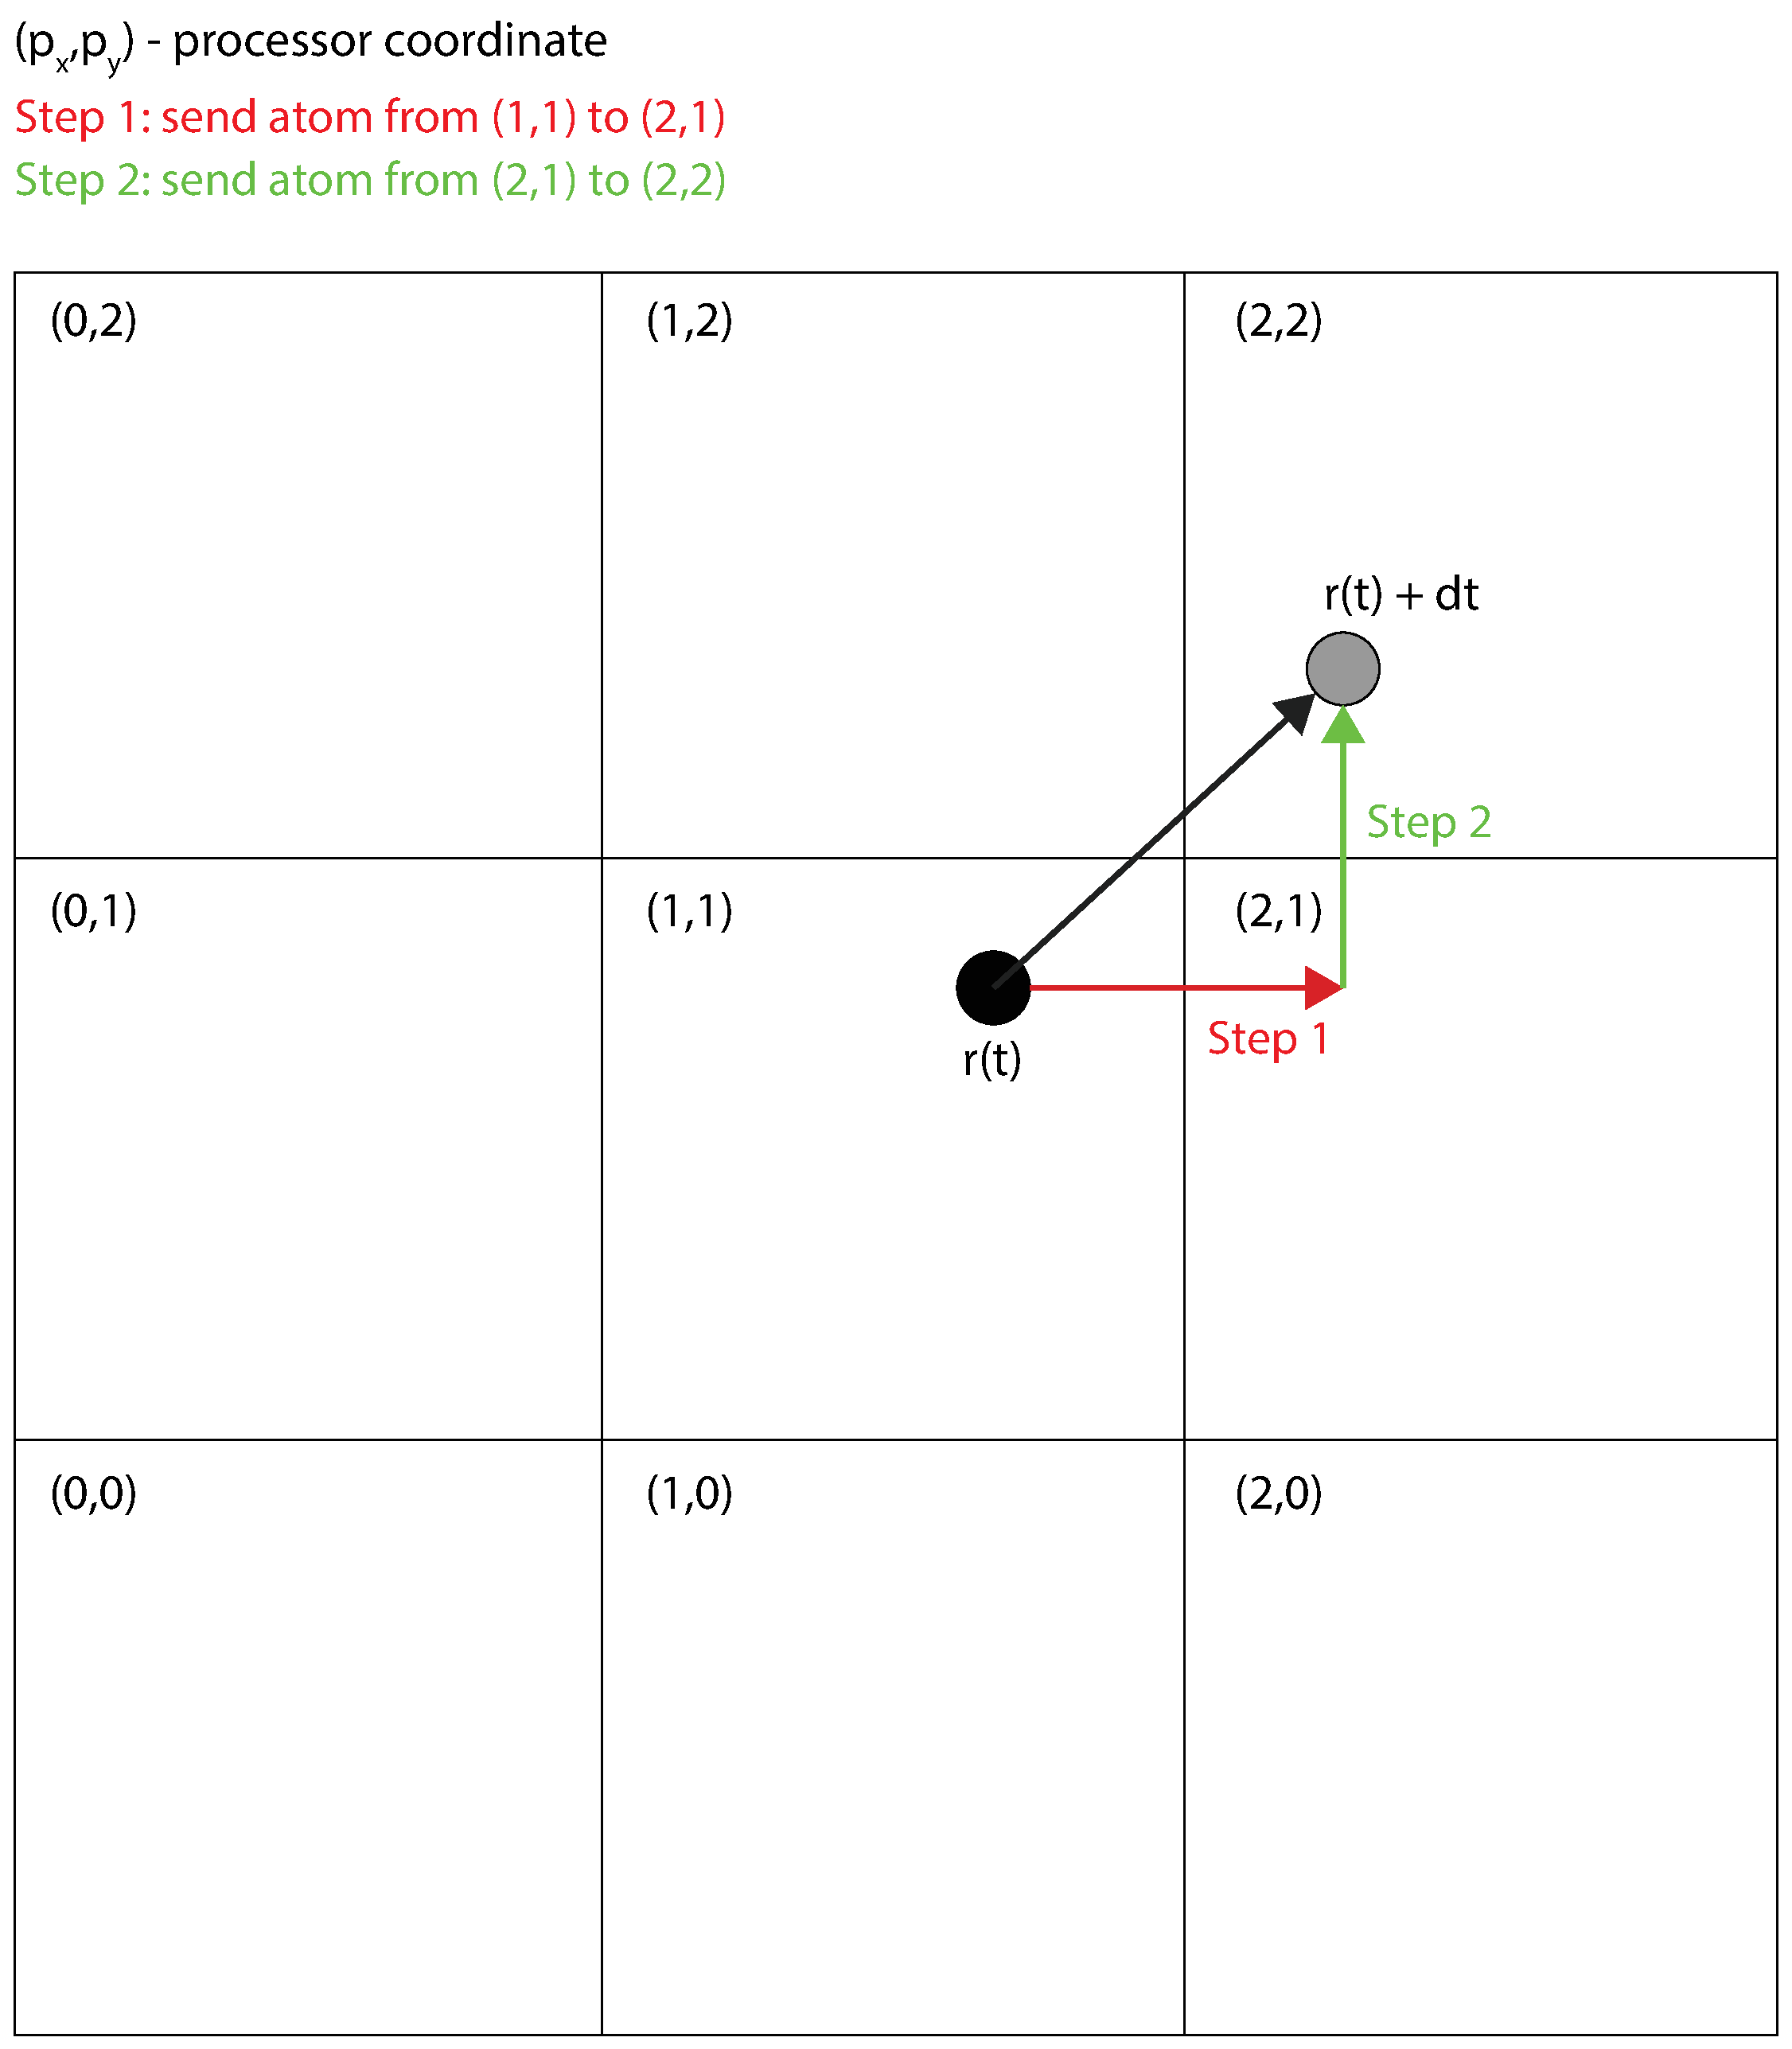
\includegraphics[width=0.7\textwidth, trim=0cm 0cm 0cm 0cm, clip]{MD/figures/parallelization_facet_technique.eps}
\end{center}
\caption{Da middle node (1,1) has 8 neighbors it need ta rap with. Each node only need ta rap wit its nearest neighbors (4 up in two dimensions, 6 up in three dimensions), cuz tha nearest neighbors can work as intermediate shiznit carriers fo' realz. An atom movin from processor (1,1) ta (2,2) will up in step 1 be busted ta (2,1), then up in step 2 be busted ta (2,2).}
\label{fig:md_parallelization_facet_technique}
\end{figure}
We only need ta know bout tha 6 nearest neighbors on each processor. Shiiit, dis aint no joke. We notice a neat detail here, periodic boundary conditions is automatically taken care of. If we again n' again n' again peep figure \ref{fig:md_parallelization_2}, our crazy asses have 4 processors up in tha $x$-direction. I aint talkin' bout chicken n' gravy biatch. Da processor ta tha \textit{right} of $(3,0,1)$ is $(0,0,1)$ if we use periodic boundary conditions. But since we use tha local coordinates on each processor, when a atom moves ta another processor, its coordinates must be \textit{shifted} so its has erect local coordinates on tha freshly smoked up processor. Shiiit, dis aint no joke. Each processor has one \textit{shift vector} per neighbor, containin tha transformation it need ta apply on tha atomz coordinates before it moved. Y'all KNOW dat shit, muthafucka! If tha atom moved all up in tha system boundary (periodic boundary conditions), tha shift vector must of course reflect all dis bullshit. 